\section{LinuX Containers}

\begin{frame}{LinuX Containers}
	\begin{columns}[T]
		\begin{column}{.6\textwidth}
			\begin{itemize}
			\item a.k.a. LXC:
				\begin{itemize}
				\item Mature technology implementation
				\item Mainline kernel support
				\item Application vs. System
				\item Active development
				\end{itemize}
			\item Components:
				\begin{itemize}
				\item \textit{Kernel features}
				\item \textit{Userspace tools}
				\item \textit{Configuration files}
				\item \textit{Template files}
				\end{itemize}
			\end{itemize}
		\end{column}
		\begin{column}{.4\textwidth}
			\begin{figure}[ht]
				\centering
				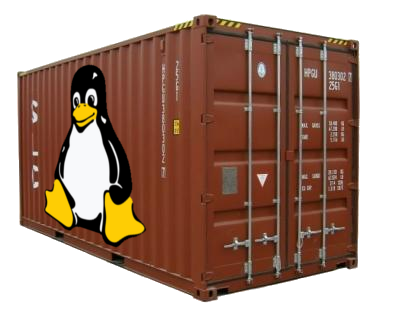
\includegraphics[width=\textwidth]{img/containers.png}
			\end{figure}
		\end{column}
	\end{columns}
\end{frame}

\begin{frame}{Kernel Support}
	\begin{columns}[C]
		\begin{column}{.6\textwidth}
			\begin{itemize}
			\setlength{\itemsep}{50pt}
			\item Namespaces:
				\begin{itemize}
				\item Abstract resources
				\item Processes see the resource as their own
				\item Isolation between namespaces
				\end{itemize}
			\item Control Groups
				\begin{itemize}
				\item Resource management among processes
				\item Hierarchical support
				\item Interaction with resource responsible structures:
					\begin{itemize}
					\item Scheduler
					\item Pager
					\end{itemize}
				\end{itemize}
			\end{itemize}	
		\end{column}
		\begin{column}{.4\textwidth}
			\begin{figure}[ht]
				\centering
				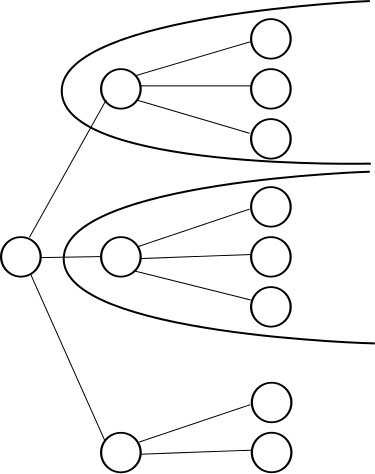
\includegraphics[scale=0.2]{img/namespaces.png}
			\end{figure}
			
			\begin{figure}[hb]
				\centering
				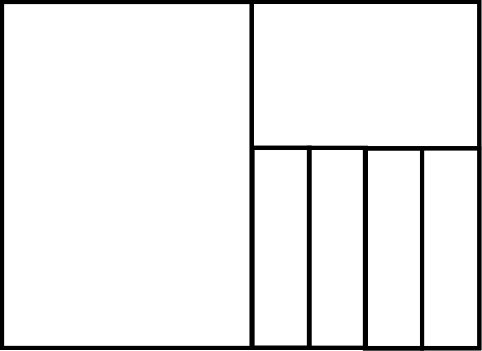
\includegraphics[scale=0.2]{img/cgroups.png}
			\end{figure}
		\end{column}
	\end{columns}
\end{frame}